\section{NFV} \label{sota:nfv}

As outlined in Section \ref{sota:5gecosystem}, the implementation of network slicing is supported by virtualization technologies, such as \acs{SDN} and \acs{NFV}, which have fundamentally transformed how networks are managed and deployed. With the growing adoption of \acs{SDN} and \acs{NFV} technologies, network functions are no longer tied to dedicated hardware instead being instantiated dynamically as software components in cloud environments. This allows operators, partners and even subscribers to create instances of their services and networks on demand~\cite{EricsonOSS}. 

This section examines the concept of \acs{NFV} and its realization through the \acf{NFV-MANO} framework. It provides an analysis of the \acs{NFV-MANO} architecture and its constituent functional blocks, detailing their respective roles and interactions in enabling the deployment and orchestration of virtualized network services.


\subsection{NFV-MANO Architectural Framework}

As previously stated, \acs{NFV} refers to the principle of separating network functions from the underlying running hardware using virtualization techniques. This approach results in \acfp{VNF}, software solutions that realize all or part of a \acf{NF} and can be deployed in the \acf{NFVI}~\cite{ETSI_GR_NFV_TERMINOLOGY_003_V1_9_1}. A \acf{NS} is then defined as the composition of one or more \acsp{NF} (\acsp{VNF} or \acsp{PNF}) and/or other \acsp{NS} to deliver \acs{E2E} services, along with the \acfp{VL} connecting them~\cite{ETSI_GS_NFV_006_V5_2_1}. The behavior of the constituting \acs{NS} is derived from the combination of its individual \acs{NF} behaviours and of the network infrastructure composition mechanism. The deployment and operational requirements of a \acs{NS} are described in a \acf{NSD}, describing the service topology, network service characteristics (e.g. \acsp{SLA}) and other depedendencies necessary for its onboarding and lifecycle management~\citep{ETSI_GS_NFV_MAN_001_V1_1_1,ETSI_GR_NFV_TERMINOLOGY_003_V1_9_1}.

The \acs{NFV-MANO} architectural framework is responsible for managing the \acs{NFVI} and orchestrating the allocation of resources needed by \acsp{NS} and \acsp{VNF}, as well as performing lifecycle management operations for \acsp{NS} and \acsp{VNF}~\citep{ETSI_GS_NFV_MAN_001_V1_1_1,ETSI_GS_NFV_006_V5_2_1}. As described in Figure \ref{fig:nfv-mano-architecture}, it is composed by the following four functional blocks~\cite{ETSI_GS_NFV_006_V5_2_1}:

\begin{itemize}
    \item \textbf{\acf{NFVO}:} responsible for the orchestration of \acs{NFVI} across multiple \acsp{VIM} and the lifecycle management of \acsp{NS} and their constituent resources. Through the \texttt{Os-Ma-nfvo} reference point, it provides an entrypoint for \acs{OSS}/\acs{BSS} to interact with the \acs{NFVO} to invoke management operations of \acsp{NSD} and to subscribe to notifications related to \acs{NSD} management changes, as specified in \acs{NFV}-SOL 005~\cite{ETSI_GS_NFV_SOL_005_V5_3_1};
    \item \textbf{\acf{VNFM}:} handles a set of management functions focused on the creation and lifecycle management of \acsp{VNF}. These include \acs{VNF} lifecycle management, \acs{VNF} configuration management, \acs{VNF} information management, \acs{VNF} performance management and \acs{VNF} fault management. It interacts with the \acs{NFVO} through the \texttt{Or-Vnfm} reference point, allowing it to invoke \acs{VNF} lifecycle management operations of \acs{VNF} instances and to subcribe to notifications regarding \acs{VNF} lifecycle changes provided by the \acs{VNFM}, as specified in \acs{NFV}-SOL 003~\cite{ETSI_GS_NFV_SOL_003_V5_3_1};
    \item \textbf{\acf{VIM}:} controls and manages the \acs{NFVI} virtual resources used by \acsp{VNF} and \acsp{VL}, regarding compute, storage and network resources. To achieve this, it exposes a \acs{NBI} for the management of \acs{NFVI} virtualized compute, storage and network resources;
    \item \textbf{\acf{WIMNFV}:} allows management of network connectivity between connectivity service endpoints, located in different sites. The \acs{WIM} performs path computation based on quality assurance factors such as jitter, round-trip time, and bandwidth requirements, establishing connectivity over the physical network~\cite{ETSI_GS_NFV_MAN_001_V1_1_1}. Within the architectural framework, the \acs{WIM} may be integrated as a part of \acs{NFV-MANO}, as depicted in Figure \ref{fig:nfv-mano-architecture}, or exist as an external component, for example, under the control of the \acs{OSS}.
\end{itemize}

\begin{figure}[htpb]
    \centering
    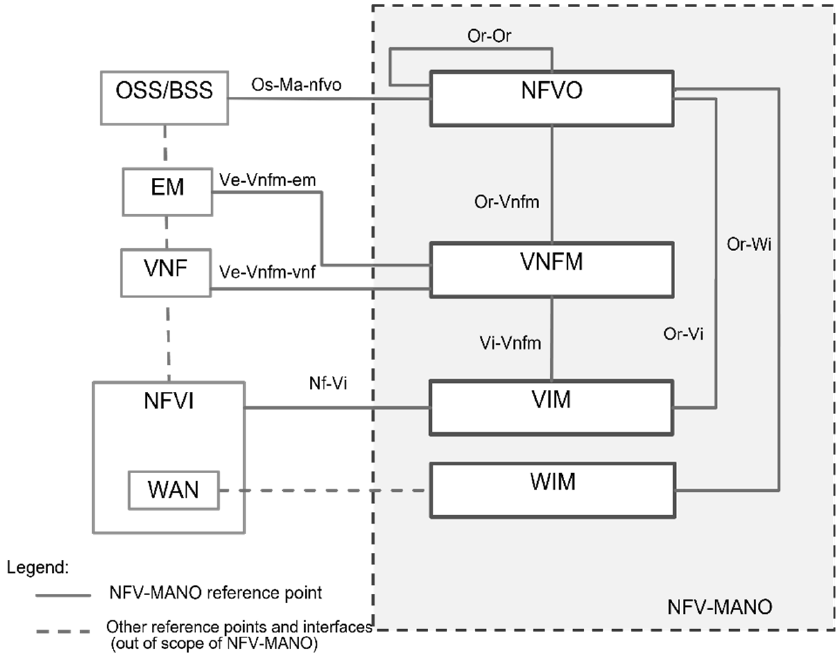
\includegraphics[width=1\linewidth]{figs/NFV-MANO-architecture.png}
    \caption{NFV-MANO architectural framework~\cite{ETSI_GS_NFV_006_V5_2_1}}
    \label{fig:nfv-mano-architecture}
\end{figure}

\clearpage

Over the years, multiple open source \acs{MANO} solutions, compliant with \acs{ETSI} \acs{NFV-MANO} have been implemented, such as the \acs{ETSI}  \acs{OSM}~\footnote{https://osm.etsi.org/}. By leveraging interfaces as the \acs{NFV}-SOL 005, it provides \acs{REST} \acsp{API} necessary for the integration with \acs{OSS}/\acs{BSS} systems, such as \acf{OSL}. This allows a more coordinated and integrated approach, yielding a series of benefits. The integration between \acs{NFV-MANO} and \acs{OSS}/\acs{BSS} systems and their benefits is further explored in Section~\ref{sec:oss:bss:nfv-mano}.




